\chapter{Theoretical Background on EDA}
\label{chap:TheoreticalBackgroundEDA}
\pagestyle{plain}
\vspace{0.5cm}

\noindent This chapter introduces the readers to Electrodermal Activities and how are they related with \gls{mer} task.
\\ \indent
First is presented a general and theoretical introduction of these \gls{eda}, how were they discovered and how are processed to have significant results.
\\ \indent
After a general introduction, some recording techniques are shown, using electrodes positioned in different parts of the body.
\\ \indent
It follow an explanation of the different techniques for preprocessing the data, as artifacts removal.
\\ \indent
At last is mentioned an explanation of the main features that can be extracted from \gls{eda} signals.

\section{Electrodermal Activity}
Already in the 80's, psychological factors related to electrodermal phenomena were observed. It became an important field of study, due to the fact its ease of obtaining a distinct \gls{edr}, the intensity of which seems apparently related to stimulus intensity and/or its psychological significance \cite{boucsein2012electrodermal}.
\\ \indent
While there is still widespread disagreement and confusion about the nature and causes of musically evoked emotions, recent studies involving real-time observation of brain activity seem to show that areas of the brain linked with emotion (as well as pleasure and reward) are activated by music listening \cite{trost2012mapping}.
\\ \indent
\gls{eda} is arguably the most useful index of changes in sympathetic arousal that are tractable to emotional and cognitive states as it is the only autonomic psychophysiological variable that is not contaminated by parasympathetic activity. \gls{eda} has been closely linked to autonomic emotional and cognitive processing, and is a widely used as a sensitive index of emotional processing and sympathetic activity.
\\
This coupling between cognitive states, arousal, emotion and attention enables \gls{eda}  to be used as an objective index of emotional states. It can also be used to examine implicit emotional responses that may occur without conscious awareness or are beyond cognitive intent (i.e., threat, anticipation, salience, novelty).

\subsection{Terminology and history}
\gls{eda} was first introduced by Johnson and Lubin in 1966 \cite{johnson1996} as a common term for all electrical phenomena in skin, including all active and passive electrical properties that can be traced back to the skin and its appendages.
\\
\gls{eda} is the property of the human body that causes continuous variation in the electrical characteristics of the skin. Historically, \gls{eda} has also been known as \gls{sc}, \gls{gsr}, \gls{edr}, \gls{pgr}, \gls{scr}, \gls{ssr} and \gls{scl}. The long history of research into the active and passive electrical properties of the skin by a variety of disciplines has resulted in an excess of names, now standardized to \gls{eda}.
\\ \indent
The use of the term \textit{response} for electrodermal phenomena suggests that there is a distinct relationship to a stimulus producing an \gls{edr}. Sometimes there are parts that cannot be traced to any specific simulation, they are called \textit{spontaneous} or \textit{non-specific} \gls{edr}.

\subsection{SCL and SCR division}
There is ample empirical evidence that electrodermal phenomena are generated by sweat gland activity in conjunction with epidermal membrane processes. Skin conductance is characterized by:
\begin{itemize}
	\item Tonic also called \gls{scl}, smooth underlying slowly changing level, it accounts for the general levels of the conductivity of the skin.
	\item Phasic, \gls{scr} rapidly changing peaks, results from momentary sympathetic activation when arousing stimuli are present.
\end{itemize}
When sweat gland activity is abolished in humans, either as a result of congenital absence, by sympathectomy, by peripheral sudomotor nerve discharge, or by pharmacological blocking, \gls{scr} and \gls{spr} are normally eliminated and \gls{scl} is reduced \cite{fowles1993electrodermal}.
\\ \indent
In the Figure \ref{fig:signal_phasic} can be seen the plot over time of an \gls{eda} signal and its decomposition in tonic and phasic parts extracted using  \href{https://github.com/MPBA/pyphysio}{pyphysio}\footnote{https://github.com/MPBA/pyphysio} library \cite{bizzego2019pyphysio} on an \gls{eda} signal. 
\begin{figure}[h]
    \centering
    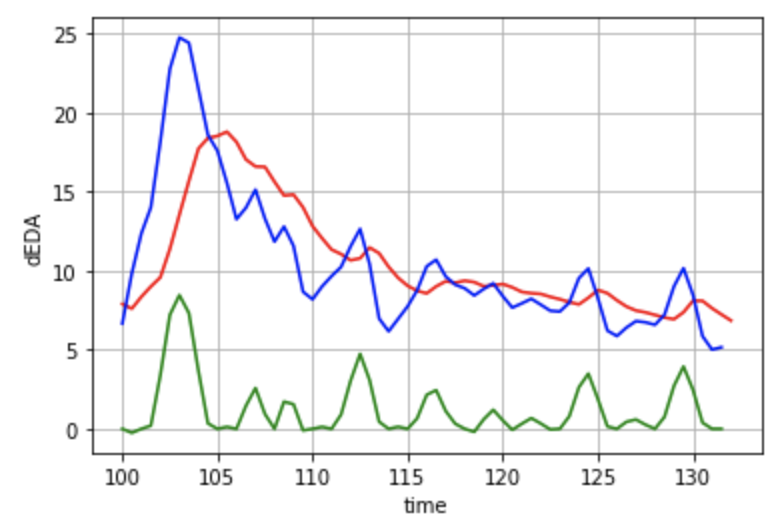
\includegraphics[width=0.7\textwidth]{signal_phasic.png} 
	\caption{Representation EDA signal (in red), driver signal (in blue) and phasic signal (in green)}
    \label{fig:signal_phasic}
\end{figure}
\\
%Another useful graph is shown in the figure \ref{fig:phasic_tonic} from \cite{hernandez2014using} that represent division between the complete signal (in blue), the tonic component (in dashed green) and the phasic component (in red).
%\begin{figure}[h]
%    \centering
%    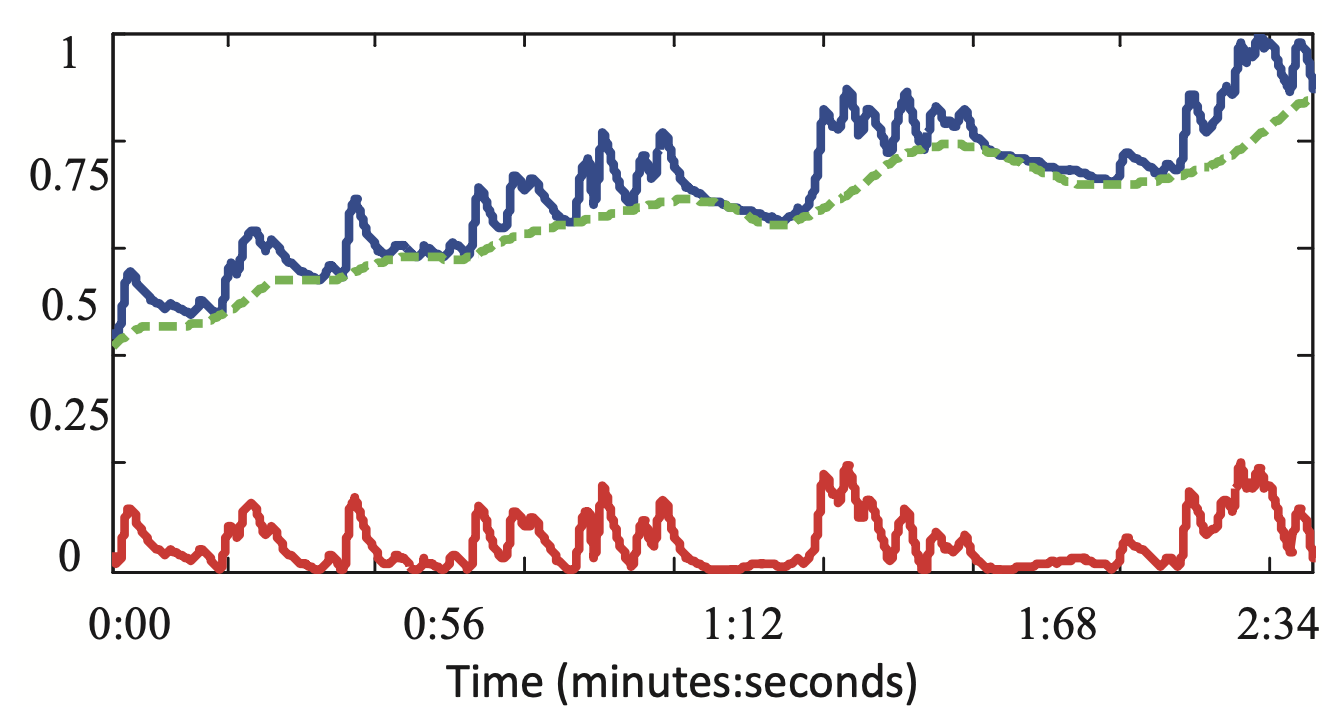
\includegraphics[width=0.8\textwidth]{phasic_tonic.png} 
%	\caption{Representation of EDA signal (in red), driver signal (in blue) and phasic signal (in dashed green) from \cite{hernandez2014using}}
%    \label{fig:phasic_tonic}
%\end{figure}
%\\
The time series of the change of \gls{sc} is characterized by a slowly varying tonic activity and fast varying phasic activity. The \gls{scr} shows a steep incline to the peak and a slow decline to the baseline. The successions of \gls{scr} usually results in a superposition of subsequent \gls{scr} as one \gls{scr} arises on top of the declining trail of the preceding one.
\\
The Figure \ref{fig:skin_conductance} from \cite{benedek2010continuous} shows a \gls{sc} data section, the upper row shows the original \gls{sc} data. The middle row shows the driver signal which results from deconvolution of the \gls{sc} data. Inter-impulse data are used to estimate the tonic part of the driver at 10-s intervals (tonic grid points). The tonic driver is used to compute the tonic \gls{sc} (see upper row). Subtraction of the tonic part from the driver results in the phasic driver (lower row). The phasic driver shows a virtually zero baseline and distinct phasic responses. 
\begin{figure}[h]
    \centering
    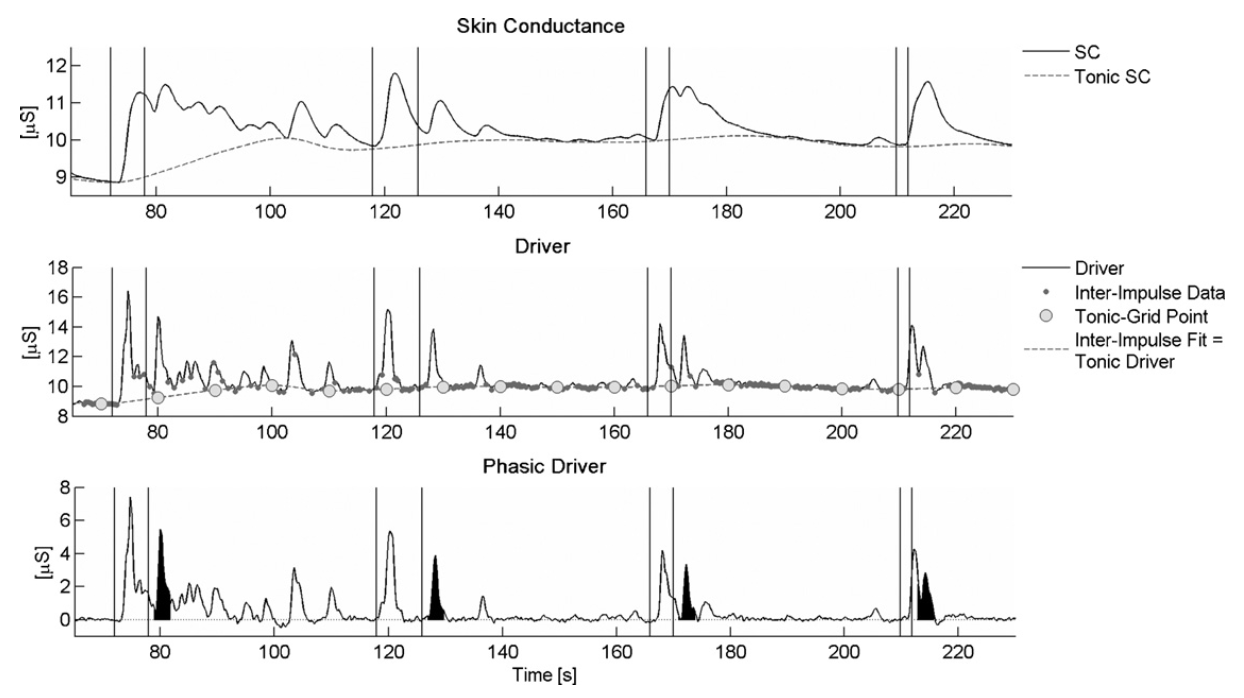
\includegraphics[width=\textwidth]{skin_conductance.png} 
	\caption{Skin conductance and phasic driver extraction from \cite{benedek2010continuous}}
    \label{fig:skin_conductance}
\end{figure}

\subsection{Decomposition algorithms and tools}
To process \gls{eda} data dividing in phasic and tonic component, in the literature, several algorithms and tools were presented.
\\ \indent
To separate the signal components, generally is designed an \gls{iir} Butterworth low-pass filter with a cut-off frequency of $0.001Hz$ (stop frequency of $1Hz$ at $-60dB$). The tonic component is then extracted from the output of the \gls{iir} filter, while the phasic component is obtained from the difference between the original signal (supplied to the \gls{iir} filter) and the tonic component.
\\ \indent
To separate phasic and tonic components, is also used an algorithm called \textit{cvxEDA}. The model of the \textit{cvxEDA} assumes that the observed \gls{scr} ($y$) is the sum of the phasic activity ($r$), a slow tonic component ($t$), and an additive independent and identically distributed zero-average Gaussian noise term ($\varepsilon$):
\begin{equation}
	y=r+t+\varepsilon
\end{equation}
Physiologically-plausible characteristics (temporal scale and smoothness) of the tonic input signal can be achieved by means of a cubic spline with equally-spaced knots every $10s$, an offset and a linear trend term:
\begin{equation}
	\label{eq:tonic_model}
	t=Bl+Cd
\end{equation}
where:
\begin{itemize}
	\item $B$ is a tall matrix whose columns are cubic B-spline basis functions
	\item $l$ is the vector of spline coefficients
	\item $C$ is a $Nx2$ matrix with $C_{i,1} = 1$, and $C_{i,2} = \dfrac{i}{N}$
	\item $d$ is a $2x1$vector with the offset and slope coefficients for the linear trend
\end{itemize}
Phasic component is the result of a convolution between the \gls{smna} $p$ and an impulse response $h(t)$ shaped as a biexponential Bateman function:
\begin{equation}
	h(t)=(e^{-t/\tau_1}-e^{-t/\tau_2})u(t)
\end{equation}
where $\tau_1$ and $\tau_2$ are the slow and the fast time constants of the phasic curve shape and $u(t)$ is the unitary step function.
\\
Referring to \cite{greco2016arousal}, the final model can be written as:
\begin{equation}
	\label{eq:EDA_model}
	y=Mq+Bl+Cd+\varepsilon 
\end{equation}
Given the EDA model \ref{eq:EDA_model}, \textit{cvxEDA} formulated the problem as a minimization problem as:
\begin{equation}
	minimize \; \dfrac{1}{2} ||Mq+Bl+Cd-y||^2+\alpha \delta ||Aq||_1+\dfrac{\gamma}{2}||l||^2_2
\end{equation}
\[subject \; to \; Aq>=0 \]
This problem can be solved using one of the many sparse-QP solvers in order to find the optimal $[q,l,d]$, than find tonic component $t$ from \ref{eq:tonic_model}.
\\ \indent
One tool is \href{http://www.musicsensorsemotion.com/2012/06/21/edatool/}{EDAtool}\footnote{http://www.musicsensorsemotion.com/2012/06/21/edatool/}. It is a function developed to preprocess \gls{eda} signal including removal of electrical noise and artifact detection. It separates also the signal in phasic and tonic components.
\\ \indent
Another tool that is able to separate signal components is \href{http://www.ledalab.de}{Ledalab}\footnote{http://www.ledalab.de}. This software aims to provide \gls{eda} analysis though two methods:
\begin{enumerate}
	\item  Continuous decomposition analysis, which performs a decomposition of \gls{sc} data into continuous signals of phasic and tonic activity.
	\item Discrete decomposition analysis, which performs a decomposition of \gls{sc} data into distinct phasic and tonic activity by means of non-negative deconvolution.
\end{enumerate}

\newpage
\section{Measurement principles}
\gls{eda} can be measured both without externally applied voltage (endosomatic method) or with application of \gls{dc} or \gls{ac} (exosomatic method). The widespread used method is the exosomatic with \gls{dc} recordings. With direct voltage, skin resistance measurements will result when current is constant, while skin conductance measurement will result when voltage is kept constant.
\\ \indent
There are some factors that should be controlled as possible sources or variance in \gls{eda} recordings, like environmental conditions as the climatic conditions and physiological factors like age, gender and ethnic differences.
\\ \indent
\gls{eda} can be measured in many different ways electrically including skin potential, resistance, conductance, admittance, and impedance. It achieves this by passing a minuscule amount of current between two electrodes in contact with the skin. The units of measurement for conductance are microSiemens ($\mu$S).

\subsection{Recording techniques}
Electrodermal recording is usually performed with two electrodes. Exosomatic techniques use two active sites, while endosomatic recording requires an active and an inactive site.
\\
Figure \ref{fig:electrode_sites} illustrate the preferred palmar recording areas for exosomatic and endosomatic \gls{eda} recordings. Sites A and B for bipolar recordings. C and D for volar electrode sites.
\begin{figure}[h]
    \centering
    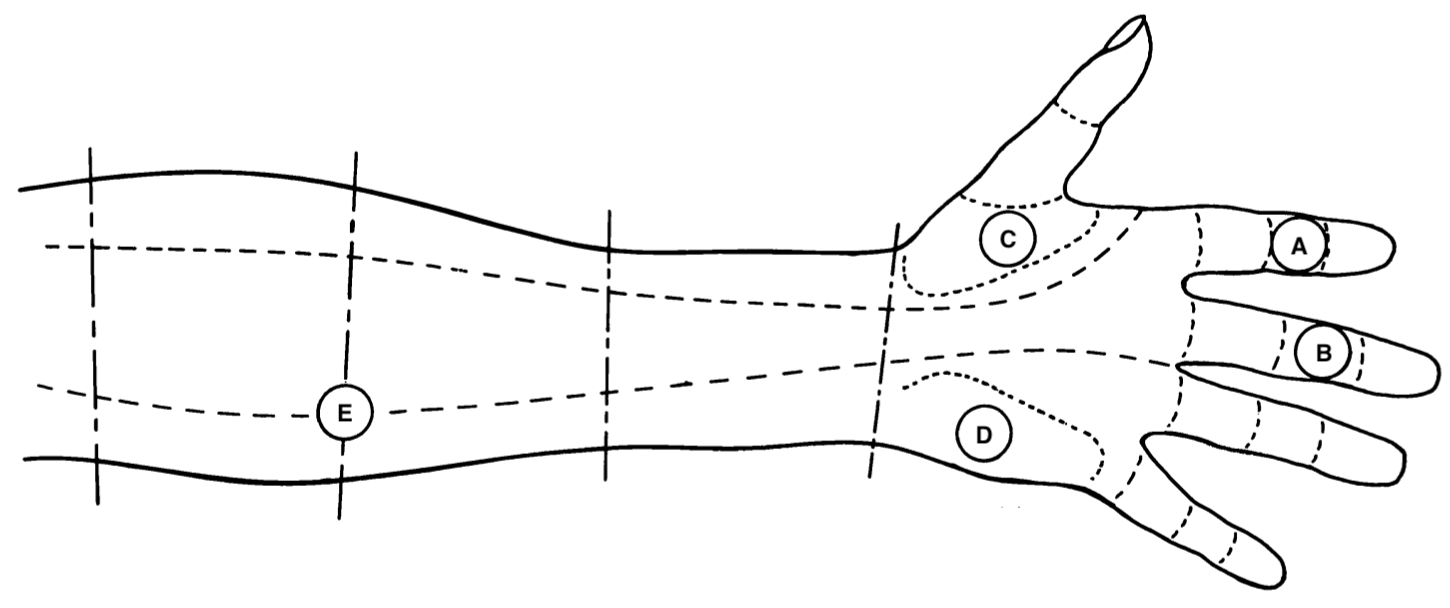
\includegraphics[width=\textwidth]{electrode_sites.png} 
	\caption{Preferred palmar recording areas for exosomatic and endosomatic EDA recordings}
    \label{fig:electrode_sites}
\end{figure}

\subsection{Wearable technologies}
During the last years, some wearable devices were made, in order to extract \gls{eda} data from a human through sensors.
\\ \indent
For example, one wearable device is from \href{https://www.empatica.com/en-eu/}{Empatica}\footnote{https://www.empatica.com/en-eu/}. Product examples can be seen in Figure \ref{fig:empatica_devices}.
\begin{figure}[h]
    \centering
    \begin{subfigure}{{0.45\textwidth}}
    		\includegraphics[width=0.8\textwidth]{e4_band.png}
    		\caption{e4}
    \end{subfigure}
    \begin{subfigure}{0.45\textwidth}
    		\includegraphics[width=0.8\textwidth]{embrace_2.png} 
    		\caption{embrace 2}
    \end{subfigure}
    \caption{Empatica wearable devices}
    \label{fig:empatica_devices}
\end{figure}
\\
Empatica has designed a system support real-world applications for seizure detection and characterization. Empatica is running a clinical trial, open to Embrace users, to collect and validate biometric signals from epilepsy patients using the Empatica Embrace watch and Alert app and compare them to e-diary seizure report information.
\\ \indent
Another device is from \href{https://www.bitbrain.com}{Bitbrain}\footnote{https://www.bitbrain.com} as in Figure \ref{fig:bitbrain}.
\begin{figure}[h]
    \centering
    \begin{subfigure}{{0.45\textwidth}}
    		\includegraphics[width=0.8\textwidth]{ring_bitbrain.png}
    		\caption{Biosignal device from Bitbrain}
    \end{subfigure}
    \begin{subfigure}{0.45\textwidth}
    		\includegraphics[width=0.8\textwidth]{ring_layout.png} 
    		\caption{Positioning the sensors}
    \end{subfigure}
    \caption{Bitbrain wearable devices}
    \label{fig:bitbrain}
\end{figure}
\\
The sensors are located on the fingers' first and second phalanges (optimal measurement points) as shown in \ref{fig:bitbrain}.
\\ \indent
Another one device is from \href{https://imotions.com}{iMotions}\footnote{https://imotions.com}. The name of the device is \textit{Shimmer3 GSR+} which monitors skin conductivity between two electrodes attached to two fingers of one hand as can be seen in Figure \ref{fig:shimmer3}.
\begin{figure}[h]
    \centering
    \begin{subfigure}{{0.45\textwidth}}
    		\includegraphics[width=0.8\textwidth]{Shimmer_3GSR.png}
    \end{subfigure}
    \begin{subfigure}{0.45\textwidth}
    		\includegraphics[width=0.8\textwidth]{Shimmer_3GSR_hand.png} 
    \end{subfigure}
    \caption{Bitbrain wearable devices}
    \label{fig:shimmer3}
\end{figure}
\\
Caused by a stimulus the sweat glands become more active, increasing moisture on the skin and allowing the current to flow more readily by changing the balance of positive and negative ions in the secreted fluid (increasing skin conductance).

\newpage
\section{EDA preprocessing}
\gls{eda} data is often captured by wearable devices, which makes the signal collected vulnerable to several types of noise. Artifacts can be generated from electronic noise or variation in the contact between the skin and the recording electrode caused by pressure, excessive movement or adjustment of the device \cite{taylor2015automatic}.
\\
They may be mistaken for a skin conductance response, and this must be avoided.
\\ \indent
Typically, as Boucsein \cite{boucsein2012electrodermal} report, the shape of an \gls{scr} lasts between $1s$ to $5s$, has a steep onset and an exponential decay and reaches an amplitude of at least $0.01\mu S$. An example of a typical \gls{scr} in Figure \ref{fig:SCR_example}.
\begin{figure}[h]
    \centering
    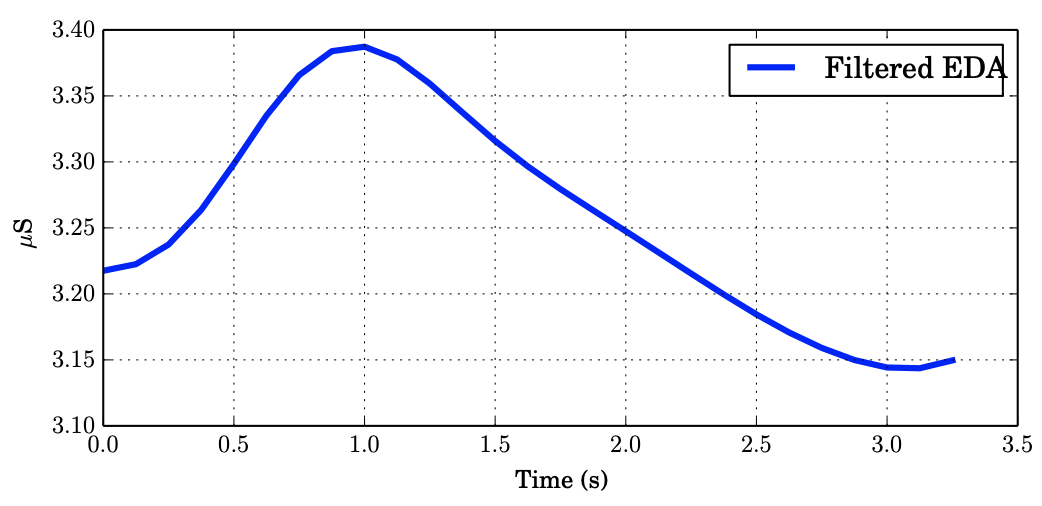
\includegraphics[scale=0.4]{SCR_example.png} 
	\caption{Example of a SCR shape}
    \label{fig:SCR_example}
\end{figure}
\\
Currently, many researchers deal with signal artifacts and noise by applying exponential smoothing or low-pass filtering.
\\
Additionally, filter cutoff frequencies are based only loosely on prior knowledge of typical characteristics of SCR shape, and vary widely study to study (from $1Hz$ to $5Hz$). The cutoff frequency ultimately chosen for a study is specific to that particular study, making generalization difficult.
\\ \indent
There are much relevant techniques that are also able to recognize and compensate for large-magnitude artifacts that can result from pressure or movement of the device during recordings.
\\
In \cite{taylor2015automatic} is presented a figure reported at Figure \ref{fig:eda_artifacts}, which shows a portion of signal that contains three artifacts, in which the fast decrease could not be produced by human physiology. Comparing the raw signal and the filtered version, the low-pass filter has not removed the artifacts.
\begin{figure}[h]
    \centering
    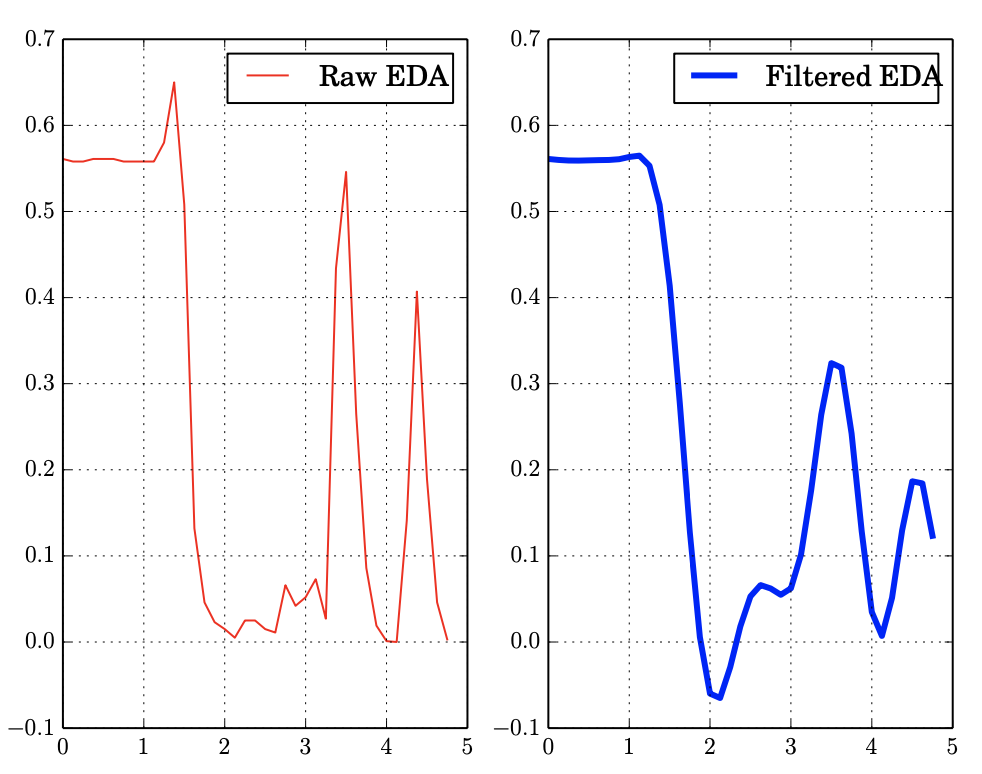
\includegraphics[scale=0.4]{eda_artifacts.png} 
	\caption{Portion of an EDA signal, the raw signal on the left in red, a $1Hz$ low-pass filter applied on the signal to the left in blue in \cite{taylor2015automatic} }
    \label{fig:eda_artifacts}
\end{figure}
\\
Some researchers, as Boucsein analysis \cite{boucsein2012electrodermal}, develop heuristic techniques for removing atypical portion of the \gls{eda} signal. Someone decide to discard portion of their data where the signal increased more than 20\% per second or decreased more than 10\% per second.
\\
In another case, a study which collected \gls{eda} from two sensors (on both the ankle and wrist) \cite{hedman2010situ} was able to detect artifacts by looking for epochs when only one of the two sensors had an abnormally low signal, or showed an unusually rapid increase or decrease.
\\ \indent
In \cite{taylor2015automatic} developed a \gls{ml} algorithm for automatically detecting \gls{eda} artifacts, providing empirical evaluation of classification performances.

\newpage
\section{EDA features}\label{EDA_features}
As for \gls{mer} analysis, also in \gls{eda} data analysis, is important to find which features need to be extracted and then which feature selection method must be carried.
\\ \indent
Emotion recognition from \gls{eda} has been commonly used for the assessment of user's experience in a variety of contexts such as recreational and games \cite{drachen2010correlation} and driving \cite{healey2005detecting}. Previous research has explored the predictive power of a diverse set of \gls{eda} features of different types, including time domain, frequency domain, and time-frequency domain features.
\\ \indent
Regarding time domain features, most usually features considered are the statistical parameters of the signal as:
\begin{itemize}
	\item Mean value: $\mu$ is the central value of a discrete set of numbers $x_1,x_2,...,x_n$, specifically, the sum of the values divided by the number of values:
		\begin{equation}
		\mu=\dfrac{1}{n} \sum_{i=1}^{n}{x_i}
		\end{equation}
	\item Standard deviation:  is a measure of the amount of variation or dispersion of a set of values:
		\begin{equation}
		\sigma=\sqrt{\dfrac{1}{n}\sum_{i=1}^{n}({x_i-\mu})^2}
		\end{equation}
	\item Kurtosis: is a measure of the "tailedness" of the probability distribution of a real-valued random variable:
		\begin{equation}
		kurt=\dfrac{\dfrac{1}{n} \sum_{i=1}^{n}{(x_i-\mu)^4}}{\sigma^4}
		\end{equation}
	\item Skewness: is a measure of the asymmetry of the probability distribution of a real-valued random variable about its mean:
		\begin{equation}
		skew=\dfrac{\dfrac{1}{n} \sum_{i=1}^{n}{(x_i-\mu)^3}}{\sigma^3}
		\end{equation}
\end{itemize}
In \cite{shukla2019feature}, as an example, were extracted the features for \gls{eda} data shown in table \ref{table:features}, where \gls{dwt} is an implementation of the wavelet transform using a discrete set of wavelet scales.
\begin{table}[h!]
	\centering
	\begin{tabular}{|l |p{0.36\textwidth} | p{0.3\textwidth}|}
		\hline
		Domain & Feature vector & Number of features\\ [0.5ex] 
		\hline\hline Time & \gls{scr} related \newline Statistical features \newline Hjorth features \newline Higher Order Crossing & 7 \newline 8 \newline 2 \newline 5 \\ 
		\hline	Frequency	 & Statistical features \newline Band power & 8 \newline 9 \\ 
		\hline	Time-Frequency & \gls{dwt} coefficients \newline SWT features \newline \gls{mfcc} \newline Statistical features \gls{mfcc} & 56 \newline 40 \newline 481 \newline 5 \\
		\hline
	\end{tabular}
	\caption{Features extracted in \cite{shukla2019feature}}
	\label{table:features}
\end{table}
\\
Other cases, researchers have focused on event-related features of \gls{eda}. They are useful when are presented to the subjects some events, stimulus, like images or sounds.
\\
Examples of event-related aspects of \gls{eda} considered in other studies are \gls{scr} amplitude, \gls{scr} peak count, mean \gls{scr} rise time, or the sum of \gls{scr} areas.
\\ \indent
Fewer researches, as \cite{shukla2019feature} remarks, has focused on the predictive power of \gls{eda} related to the frequency domain. The frequency domain analysis has shown superior capability for the gradient component's detection of individual \gls{scr}.
\\
Due to the different rate of physiological process, \gls{eda} signals vary significantly with the frequency \cite{ghaderyan2016efficient}.
\\
Frequency oscillations of \gls{eda} signals can be divided into different frequency sub-bands to analyze it. Indeed previous researchers has considered statistical aspects (variance, range, signal magnitude area, skewness, kurtosis, harmonics summation) and spectrum power of five frequency bands, as well as their minimum, maximum, and variance.
\\ \indent
As for audio, also for \gls{eda} data, after constructing a feature matrix, need to apply an algorithm of feature selection to improve data reliability.
\\ \\
Some examples of feature selection could be:
\begin{itemize}
	\item \gls{jmi}: focuses on the increasing complementary information between features.
	\item \gls{cmim}: it can properly identify truly redundant features and noisy features, and gives preference to informative, uncorrelated features.
	\item \gls{disr}: a normalized variant of \gls{jmi}.
\end{itemize}
In general it is not known which features are most appropriate for emotion recognition from \gls{eda} and previous works have made limited contributions on a systematic comparison of \gls{eda} features.
\\
In \cite{shukla2019feature} there is a table showing various features extracted for \gls{eda} signals already presented in Table \ref{table:features} with also references in the literature.